
\section{Various tensor representations}\label{sec:varioustensorrepresentations}
%
In this section, we give some tips on how to change between the different representations of a tensor. We use the metric tensor $\metric$ to develop the methods and then we apply them to some examples.

\theme{Slot representation:} by definition, $\metric$ takes two vectors. Then, its slot representation is straightforward: 
%
\begin{equation*}
  \metric = \metric\vat{\vslot,\vslot}\,.
\end{equation*}

\theme{Components:} now, choose a basis $\bset{\tbvec\mu}{\mu = 0}{3}$ and its dual $\bset{\tbcov\mu}{\mu = 0}{3}$. To find $\metric$ components on the give basis, plug in the basis element into $\metric$ slots:
%
\begin{equation*}
  \metric\vat{\tbvec\mu,\tbvec\nu} = \tmetric\mu\nu\,.
\end{equation*}
%
Note how the positions of the indices in the rhs match the positions of the indices in the lhs, to respect Einstein's summation convention (ESC).

\theme{Projection:} write down $\metric$ components $\tmetric\mu\nu$ and match their indices with the tensor product of the basis elements, respecting ESC:
%
\begin{equation*}
  \metric = \tmetric\mu\nu\,\tbcov\mu\tprod\tbcov\nu\,.
\end{equation*}
%
Note that, since $\metric$ accepts vectors, it behaves as a covector! Thus, its components are written as subscripts.

Finally, these results match \cref{eq:metricinvmetricidtensorexpansiononabasis}.

\begin{example}
  Say that we want to construct the various representations of the inverse metric tensor $\invmet$, but beginning with its components, $\tinvmet\mu\nu$.
\end{example}
%
\begin{solution}
  \theme{Projection:} choose a basis and its dual. Then, for the tensor, form the basis with appropriate tensor products of its elements using the tensor components and ESC:
  %
  \begin{equation*}
    \invmet = \tinvmet\mu\nu\,\tbvec\mu\tprod\tbvec\nu\,.
  \end{equation*}
  %
  Note that $\tinvmet\mu\nu$ has two superscript indices, thus two covectors (with subscripts) must be given to match the superscript ones.
  
  \theme{Arguments:} with the components $\tinvmet\mu\nu$, it is possible to write the argument list of $\invmet$, by taken ESC into account:
  %
  \begin{equation*}
    \tinvmet\mu\nu = \invmet\vat{\tbcov\mu,\tbcov\nu}\,.
  \end{equation*}
  
  \theme{Slot representation:} with the argument list, the slot representation follows immediately:
  %
  \begin{equation*}
    \invmet\vat{\cslot,\cslot} = \invmet\vat{\tbcov\mu,\tbcov\nu}\,.
  \end{equation*}
  
  Finally, it can be seen that $\invmet$ behaves as a vector, since it accepts two covectors as arguments. This is in accordance with the definition of $\invmet$.
\end{solution}

\begin{example}
  Consider a $\torder 21$ tensor $t$ with components $\tensor{t}{^\mu_\nu_\lambda}$. Find the different representations of $t$.
\end{example}
%
\begin{solution}
  Writing down the different representations is straightforward by keeping in mind to place the index in the same position at both sides of the equations and ESC.

  \theme{Argument list:} $\tensor{t}{^\mu_\nu_\lambda}\implies t\vat{\tbcov\mu,\tbvec\nu,\tbvec\lambda}$.
  
  \theme{Projection:} $t\vat{\tbcov\mu,\tbvec\nu,\tbvec\lambda}\implies \tensor{t}{^\mu_\nu_\lambda}\,\tbvec\mu\tprod\tbcov\nu\tprod\tbcov\lambda$.
  
  \theme{Slot representation:} $t\vat{\tbcov\mu,\tbvec\nu,\tbvec\lambda}\implies t\vat{\cslot,\vslot,\vslot}$.
\end{solution}


\subsection{Graphical representation of tensors}
%
\begin{figure}[b]
  \capstart
  \centering
  %
  \begin{subfigure}{0.55\textwidth}
    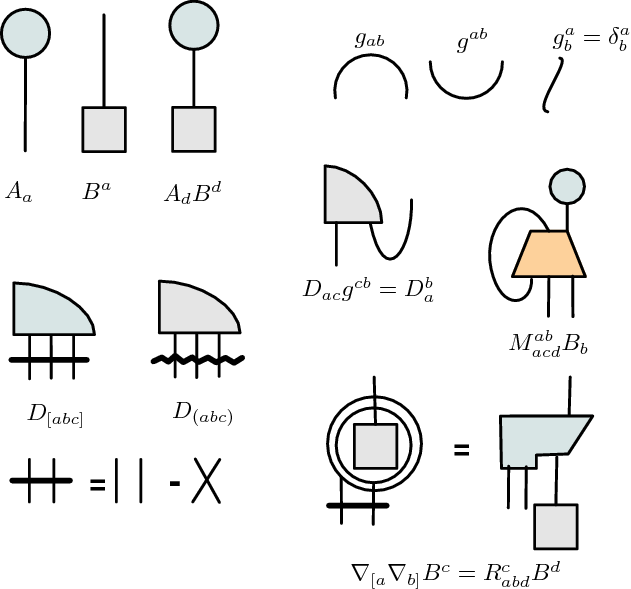
\includegraphics[width=\textwidth]{./graph/penrose}
    \caption{Penrose notation}
    \label{fig:penrosenotationfortensors}
  \end{subfigure}
  %
  %\quad
  %
  \begin{subfigure}{0.60\textwidth}
    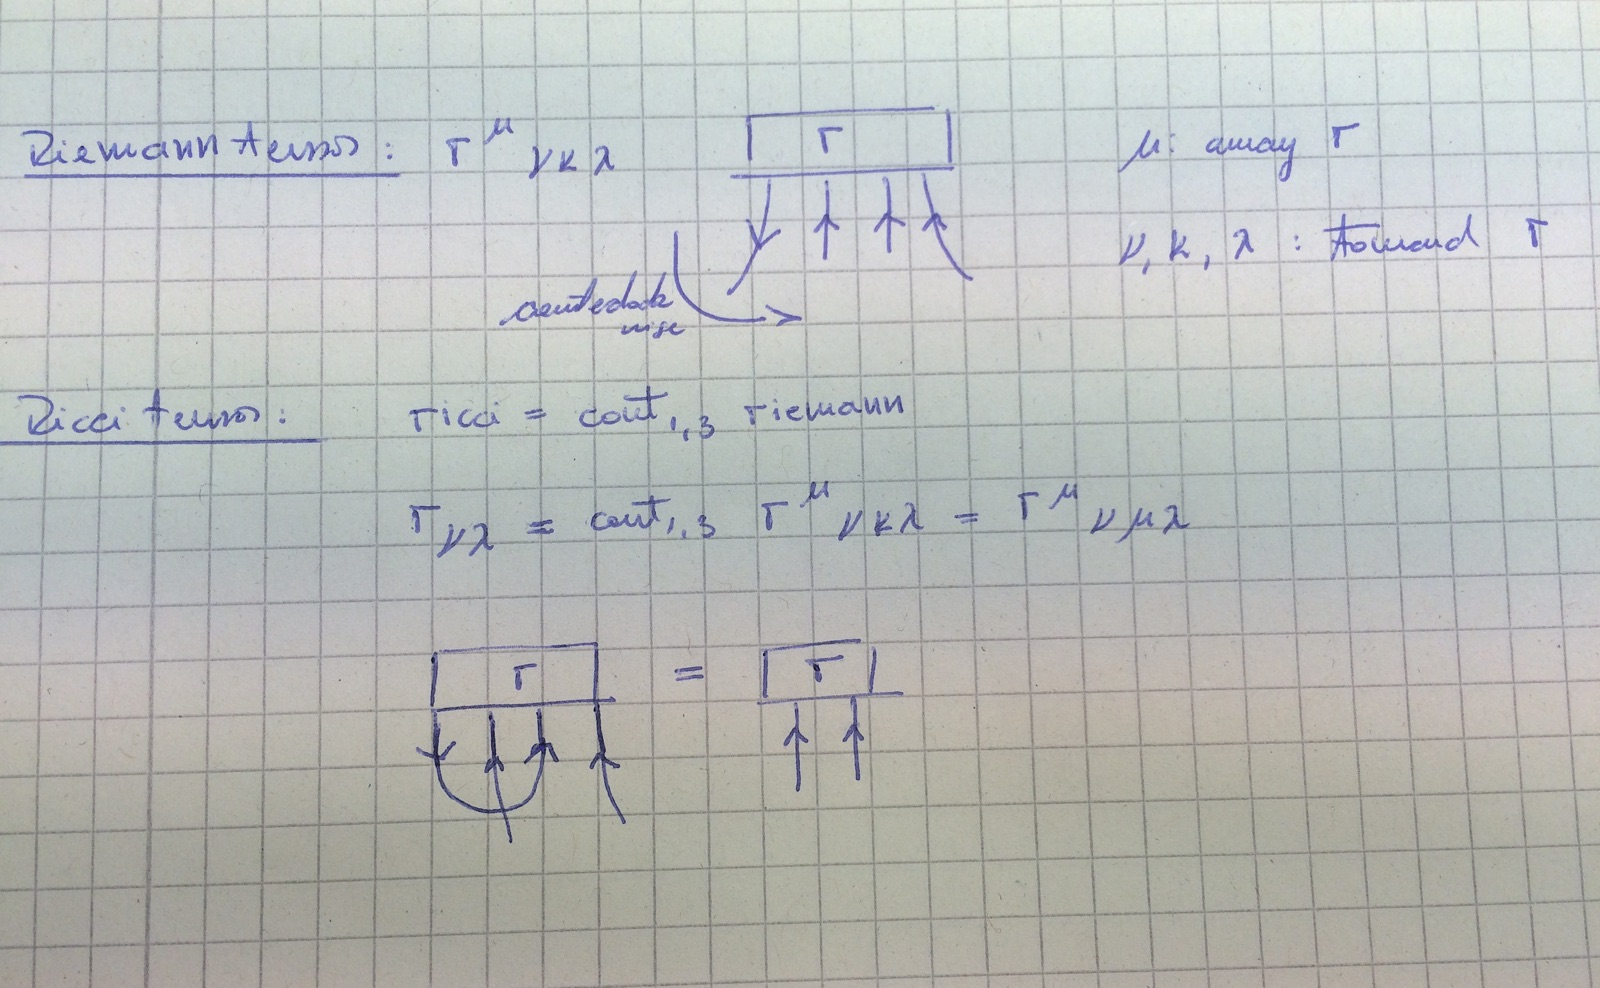
\includegraphics[width=\textwidth]{./graph/cvitanovic}
    \caption{Cvitanovic notation}
    \label{fig:cvitanovicnotationfortensors}
  \end{subfigure}
  %
  \caption{Penrose and Cvitanovic's graphical notation for tensors. Penrose's notation relies on shapes and wires: tensors are represented by prescribed shapes and indices by arrows: contravariant indices spring from above the figure; while covariant from below. Cvitanovic's notation, on the other hand, uses arrows springing for tensors: contravariant indices are represented by arrows pointing away from the tensor; while covariant, toward the tensor.}
  \label{fig:graphicalnotationfortensors}
\end{figure}
%
Cvitanovic's graphical notation for tensors: Penrose's notation modified by \cite[p.27]{cvitanovic:2008}], shown in \cref{fig:graphicalnotationfortensors}:
%
\begin{itemize}
  \item tensors are enclosed by figures like boxes or circles;
  \item arrows point \emph{away from the figure for the upper indices} (vector indices or contravariant indices); while \emph{toward the figure for the lower indices} (covector indices or covariant indices);
  \item diagrammatic notation must indicate which in (out) arrow correspond to the first upper (lower) index of the tensor;
  \item indices are read \emph{counterclockwise} around the vertex.
\end{itemize}

\theme{Mnemotecnic.} Vectors can be thought of a \scare{hot} spots: they release energy to space; therefore, its arrows point away from the box. Covectors can be thought of a \scare{cold} spots: they accept energy from space; thus, its arrow point toward the box.


\subsection{Untraditional ways of solving problems}
%
Index notation, slot notation, ESC, and diagrammatic notation for tensors and ESC can be very effective in problem solving. Some examples, below.

\theme{Linear momentum.} Let's get right the equation of linear of momentum $\lmom$ for a particle with mass $m$ moving with velocity $\vel$.

We know that velocity is a vector, by definition: $\vec\vel$. Thus it has a covector slot: $\vec\vel\vat\cslot$, which means that its components are $\vec\vel\vat{\tbcov\mu}\implies\tvec\vel\mu$. On the other hand, from Lagrangian mechanics, we know that momentum is a covector. Thus, $\cov\lmom\implies\cov\lmom\vat\vslot\implies\cov\lmom\vat{\tbvec\mu}\implies\tcov\lmom\mu$.

